\documentclass{article}
\setcounter{tocdepth}{4}
\setcounter{secnumdepth}{4}
\usepackage[hidelinks]{hyperref}
\usepackage{pgfplots}
\usepackage{pdfpages}


\usepackage{verbatim,lmodern,amsmath,Asymptote,ctex,tikz,graphicx,subcaption,enumitem}
\usepackage[left=5cm,right=5cm,top=3cm,bottom=3cm]{geometry}
\pgfplotsset{width=7cm,compat=1.16}
\begin{document}
	\tableofcontents
	\section{introduction}
	\subsection{古典密码}
	\par\indent
	\subsubsection{私钥加密}
	\par\indent
	加密双方使用相同密钥进行加密和解密。
	\par\indent
	\begin{align}
		cipher &= Enc_k(message) \\
		message &= Dec_k(cipher)
	\end{align}
	\subsubsection{柯克霍夫原则(Kerckhoffs’ principle)}
	加密方法公开,密钥私密。有如下优点
	\begin{enumerate}
		\item 易于保存和修改
		\item 易于加密双方交换必要信息(密钥)
		\item 大规模使用中,加密方法公开才易于软硬件的实现
	\end{enumerate}
	\subsubsection{凯撒密码(Caesar’s cipher)}
	\par\indent
	凯撒密码是一种古老的加密方法,其本质是移位密码。通过将字母在字母表中的
	顺序向后移动3位,如遇到结尾,则跳到开头,得到的新字母便为该字母对应
	的密文字母,例:$d=enc_{Caesar}(a)=d$,$c=enc_{Caesar}(z)$;
	$ch \in{\left\{0,...,25\right\}}$
	则$enc\_ch = ch + 3 \mod 26 $,$ch \in{\left\{0,...,25\right\}}$。
	\subsubsection{移位密码}
	\par\indent
	凯撒密码变体,$ch \in{\left\{0,...25\right\}}$,
	$enc\_ch =ch + k \mod 26$,$k \in{\left\{0,..,25\right\}}$,移位密码
	仅有26个密钥。
	\par\indent
	\subsubsection{移位密码的破解方法}
	\paragraph{人工破解方法}
	\par\indent
	对于凯撒密码,向前移三位便可以得到明文,而对于移位密码,它的移位
	可以通过穷举26个密钥得到,并且过程中需人工辅助判断来选择其中一个
	有意义的作为明文消息。
	\paragraph{机器破解方法}
	\par\indent 
	机器破解方法是因为在人类交流的语言中,各个
	字母出现的频率并不相同,如下图所示:\\
	\pgfplotsset{width=16cm,height=8cm}
	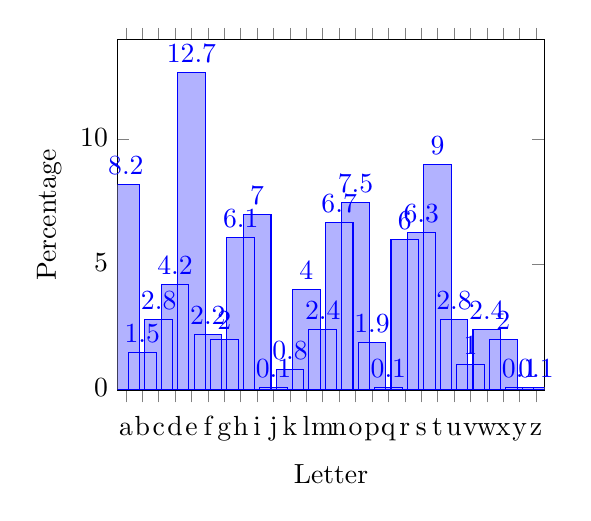
\begin{tikzpicture}
		\begin{axis}[
			nodes near coords,   
			ybar,
			ymax=14,
			enlarge y limits={value=0.01,lower},
			enlarge x limits =0.02,
			ylabel=Percentage,
			xlabel=Letter,
			symbolic x coords={
				a,b,c,d,e,f,g,h,i,j,k,l,m,n,o,p,q,r,s,t,u,v,w,x,y,z
			},
			xtick=data,
			typeset ticklabels with strut,
			]
			\addplot coordinates {
				(a,8.2) (b,1.5) (c,2.8) (d,4.2) 
				(e,12.7) (f,2.2) (g,2.0) (h,6.1)
				(i,7.0) (j,0.1) (k,0.8) (l,4.0) (m,2.4) (n,6.7)
				(o,7.5) (p,1.9) (q,0.1) (r,6.0) (s,6.3) (t,9.0)
				(u,2.8) (v,1.0) (w,2.4) (x,2.0) (y,0.1) (z,0.1) 
			};
		\end{axis}
	\end{tikzpicture}
	由于这个特性的存在,人们可以统计密文字母的出现频率来求解明文。这种
	破解方法不依赖于人的判断,并且应用范围更广。
	
	\subsubsection{仿射密码}
	\begin{equation}
		enc\_ch = ch * k + b \mod 26 \qquad 且 gcd(k,26) =1;
	\end{equation}
	\paragraph{仿射密码的破解}
	\par\indent 仿射密码可以移位密码的方法二来破解。
	
	\subsubsection{单表代换(The mono-alphabetic substitution cipher)}
	\par\indent
	$y=f(x)$,$x \in{\left\{a,...,z\right\}}$, 
	$y \in{\left\{a,...,z\right\}}$,其中
	函数f是一个单射和满射。单表代换的密钥空间很大,
	大小为$A_{26}^{26} = 26 ! \approx 2^{88}$,
	这是一个非常大的秘钥空间,很难在短时间内遍历完
	整个秘钥空间。上文提到的凯撒密码,移位密码及仿
	射密码都属于单表代换。
	\paragraph{单表代换的破解方法}
	\par\indent
	单表代换无法隐藏不同字母在人类语言中使用频率不同的
	事实,并且无法改变$Percentage(x) =Percentage(f(x))$这一
	事实,因此,上文提到的频率统计攻击方法能完全攻破单表代换加
	密的密文,密钥空间再大也没用。
	
	
	\subsubsection{多表代换($The\; Vigen\grave{e}re\;cipher)$}
	\par\indent
	多表代换也可以称作维吉利亚加密,
	它能够将同一字母在不
	同的位置上映射到不同的密文字母上,使得单表代
	换的破解方法不再直接适合于多表代换。下表实例中
	key为密钥,周期为$4$,字母${a...z}$代表将明文字母
	移动${0...25}$,最后再将密文字母转换成大写就完成了
	整个加密过程。
	\\
	\begin{tabular}{lr}
		\hline
		Plaintext:&\texttt{tellhimaboutme}\\
		Key(repeated):&\texttt{cafecafecafeca}\\
		Ciphertext:&\texttt{VEQPJIREDOZXOE}\\
		\hline  
	\end{tabular}
	\paragraph{多表代换的破解方法}
	\par\indent
	%多表代换的攻击方法需要求解Key的周期,从cipher中取一个
	%字母\alpha ,然后找到所有\alpha 出现的位置,求相临两个
	%\alpha 的间距,它们的公倍数即为key的长度或key长度的整数倍
	,取该公倍数为T,以T为周期,密文中的任意一个位置$t$,对所有
	的$\left\{{k*T+t,k\in Z}\right\}$这些字符组成的集合具有单表代换的性质,
	可按单表代换的攻击方法进行破解。
	\subsection{现代加密原则}
	\subsubsection{形式化定义}
	\paragraph{攻击模型}
	\begin{enumerate}
		\item \textit{唯密文攻击(Ciphertext-only attack)} 
		\\攻击者只能取得密文,从密文推断原信息 
		\item \textit{己知明文攻击(Known-plaintext attack)}
		\\ 已经知道一些明文和密文来破解新的密文
		\item \textit{选择明文攻击(Chosen-plaintext attack)}
		\\ 攻击者能得到他想要的明文的密文
		\item \textit{选择密文攻击(Chosen-ciphertext attack)}
		\\ 选择一些密文来获得其原文
	\end{enumerate}
	\paragraph{精确假设(Precise Assumptions)}
	\begin{enumerate}
		\item \textit{假设的有效性(Validation of assumptions)}
		\\假设无法证明正确,却很难被驳倒
		\item \textit{方案比较}
		\\ 比较假设来判断方法的优劣和等价性
		\item \textit{假设的必要性}
		\\ 基于假设,如果该假设命题被破解,便意味着加密方法的失效
	\end{enumerate}
	\paragraph{安全性证明和现实安全}
	\par\indent
	现代加密体系建立在严格的数学基础上,但是其仍有艺术性的一面
	,仍可以构造新的数学假设,新的原始基础来发挥创造性。
	\begin{comment}
		\section{完善保密}
		
		\subsection{香农}
		\begin{enumerate}
			\item 评价安全体,计算安全性
			\item 混乱扩散
			\item 乘积密码体制
		\end{enumerate}
		$P\left[x|y\right] = P\left[x\right]$\\
		左边后验,右边先验
		贝叶斯公式
		\begin{equation}
			P[x|y] =\frac{P[y|x]P[x]}{P[y]}
		\end{equation}
		一次一密
	\end{comment}
\end{document}

